\documentclass[a4paper,12pt]{report}

\usepackage[top = 1in, bottom = 1in, left = 1in, right = 1in]{geometry}
\usepackage{titlesec}
\usepackage{graphicx}
\usepackage{fancyhdr}
\usepackage{amsmath, amsthm, amssymb, wasysym}
\usepackage{lastpage}
\usepackage[subrefformat=parens,labelformat=parens]{subfig}
\usepackage{lscape}
\usepackage[none]{hyphenat}
\usepackage{setspace}
\usepackage{xcolor}
\usepackage{float}
%\usepackage{listing}
\usepackage{tocstyle}
%\usepackage{epstopdf}                                      % EPS graphic support
\usepackage{fontspec}
\usepackage[newfloat]{minted}                                     % Code snippets
\usepackage{caption}
\usepackage{bm}                                              % Bold maths symbols
%\usepackage{enumerate}
\usepackage{enumitem}
%\usepackage{cleveref}
\usepackage{booktabs}
\usepackage{array}
\usepackage{longtable}
\usepackage{multirow}
\usepackage[bottom, perpage]{footmisc}

\bibliographystyle{preamble/IEEEtran/bibtex/IEEEtran}

% Title Spacing
\titlespacing\section{0pt}{12pt plus 4pt minus 2pt}{-5pt plus 2pt minus 2pt}
\titlespacing\subsection{0pt}{12pt plus 4pt minus 2pt}{-5pt plus 2pt minus 2pt}
\titlespacing\subsubsection{0pt}{12pt plus 4pt minus 2pt}{-5pt plus 2pt minus 2pt}

% Lists
\setlist{itemsep=1pt, topsep=1pt}
\renewcommand{\labelitemii}{$\circ$}
\renewcommand{\labelitemiii}{\textendash}
\renewcommand{\labelitemiv}{$\sqbullet$}

\newlist{RM}{enumerate}{5}
\setlist[RM,1]{label=RM-\arabic*:, ref=RM-\arabic*}
\setlist[RM,2]{label=RM-\arabic{RMi}.\arabic*:, ref=\arabic{RMi}.\arabic*}

\newlist{RE}{enumerate}{5}
\setlist[RE,1]{label=RE-\arabic*:, ref=RE-\arabic*}
\setlist[RE,2]{label=RE-\arabic{REi}.\arabic*:, ref=RE-\arabic{REi}.\arabic*}

\newlist{RS}{enumerate}{5}
\setlist[RS,1]{label=RS-\arabic*:, ref=RS-\arabic*}
\setlist[RS,2]{label=RS-\arabic{RSi}.\arabic*:, ref=\arabic{RSi}.\arabic*}

\newlist{TEST}{enumerate}{5}
\setlist[TEST,1]{label=TEST-\arabic*:, ref=TEST-\arabic*}
% Commands
\providecommand{\e}[1]{\ensuremath{\times 10^{#1}}}       % Scientific Notation!
\providecommand{\eoc}{\ensuremath{_{\slash \slash \slash}}} % End of Calculation Symbol!
\providecommand{\subheading}[1]{\textit{#1}}

% Tables
\newcolumntype{L}[1]{>{\raggedright\let\newline\\\arraybackslash\hspace{0pt}}m{#1}}
\newcolumntype{C}[1]{>{\centering\let\newline\\\arraybackslash\hspace{0pt}}m{#1}}
\newcolumntype{R}[1]{>{\raggedleft\let\newline\\\arraybackslash\hspace{0pt}}m{#1}}

\parskip = 6mm
\parindent = 0mm
\renewcommand{\headrulewidth}{0pt}
\rhead[]{\thesection}
\lhead[\thechapter]{}

% hyperref
\usepackage[bookmarks         = true     ,%
            bookmarksnumbered = true     ,%
            setpagesize       = false    ,%
            colorlinks        = true     ,%
            linkcolor         = black    ,%
            urlcolor          = black    ,%
            citecolor         = black    ,%
            pdfpagelayout     = OneColumn,%
            pdfstartview      = FitH		 ,%
            driverfallback    = dvipdfm]{hyperref}
            
% fonts
\setmonofont{Fira Code}[Scale=MatchLowercase]
            
% minted
\newenvironment{code}{\captionsetup{type=listing}}{}
\SetupFloatingEnvironment{listing}{name=Snippet}

\definecolor{mintedBg}{rgb}{0.94,0.94,0.94}
\setminted[]{%
  breaklines 	= true,%
  autogobble 	= true,%
  bgcolor			= mintedBg,%
  linenos			= true,%
}
%\usemintedstyle{pastie}
            


\begin{document}
 
% Coverpage
\thispagestyle{empty}
{\Huge \begin{center}

% Title
Development of a Mars Curiosity Rover Simulator
\vskip 5mm
\hrule 

% Subtitle
{\Large A working model intended for modern space science education and outreach}
\end{center}}

\vskip 5mm
\begin{center}

\includegraphics[scale = 0.3]{uctLogo.png}
\end{center}

\vskip 5mm
\begin{center}
{\large
\textbf{Prepared by:}
\vskip 0.01mm
\textbf{\LARGE Sean Wood}\\
Dept. of Electrical and Electronics Engineering\\University of Cape Town
}
\end{center}

\vskip 10mm
\begin{center}
{\large
\textbf{Prepared for:}
\vskip 0.01mm
\textbf{\LARGE Professor Peter Martinez}\\
Dept. of Electrical and Electronics Engineering\\University of Cape Town
}
\end{center}


\vskip 10mm
\begin{center}
Submitted to the Department of Electrical Engineering at the University of Cape Town in partial
fulfilment of the academic requirements for a Bachelor of Science degree in Mechatronics

\end{center}


\vskip 5mm
\begin{center}{\bf \today}
\end{center}

% Empty Page
\newpage
\thispagestyle{empty}
\mbox{}
\newpage

\pagenumbering{roman}
\addcontentsline{toc}{section}{Terms of Reference}
{\Large Terms of Reference}\\
\hrule

\section*{Title}
  Development of a Mars Curiosity Rover Simulator
\section*{Description}
  Our knowledge of the planet Mars has been greatly expanded by several rovers that have landed on the planet over the past twenty years. The most capable of these is the \textit{Curiosity} Rover, which is currently exploring the surface of Mars. In an attempt to generate awareness of the effort put into planetary exploration, the project involves the development of a model of the \textit{Curiosity} Rover which replicates some of the control experiences involved in operating a rover of this type.
  
\section*{Deliverables}
  
\section*{Skills and Requirements}
  Mechanical Design, Software and Electronics Interfacing and Programming.
  
\section*{Area}
  Space Science and Technology


\newpage
%\onehalfspacing
\thispagestyle{empty}
\vskip 40mm

% Please leave the declaration as it is (Standard UCT declaration).
{\Large Declaration}\\
\hrule

\vskip 10mm
\begin{enumerate}
\item I know that plagiarism is wrong. Plagiarism is to use another's work and pretend that it is one's
own.
\item I have used the IEEE convention for citation and referencing. Each contribution to, and quotation in,
this report from the work(s) of other people has been attributed, and has been cited and
referenced.
\item This report is my own work.
\item I have not allowed, and will not allow, anyone to copy my work with the intention of passing it off
as their own work or part thereof.
\end{enumerate}
\vskip 10mm
Signature:\ldots\ldots\ldots\ldots\ldots\ldots\ldots\ldots\ldots 
\\M. S. T\v soeu 		% Chante this line to your name.
\vskip10mm
Date:\ldots\ldots\ldots\ldots\ldots\ldots\ldots\ldots\ldots\ldots .


\fancyfoot[C]{\thepage}

\newpage

\pagestyle{plain}

\addcontentsline{toc}{section}{Acknowledgements}
{\Large Acknowledgments}\\
\hrule

No project such as this one could have come into existence without the effort from many other people. Here, I would like to acknowledge those who have given up some of their time and expertise to help me put this project together, from the start where it was a seemingly ambitious idea, to now where everything actually works. The success of this project can only be due to the support structure that I have, and for that I am truly grateful.

I'd like to firstly thank my project supervisor, Prof. Peter Martinez, for his guidance in the project as well as in the field of space science in general. It is refreshing to work with an expert in the field willing to recognise and explore others' ideas for the better of the project.

I'd like to thank Justin Pead from the UCT's Whitelab for facilitating all the extraordinary electrical and mechanical requests that came about from the project. I am thankful for the guidance he has given me in many projects during my undergraduate degree.

I'd like to thank the members of the SpaceLab, in which I worked on this project, for checking up on me almost everyday. The SpaceLab was an incredible place in which to work and everyone was supportive of the work that I was doing, ready to get up and help me out whenever I needed it.

I'd like to thank my classmates from all corners of the electrical department. I learnt from them that this degree was not one walked alone, and this was a collective realisation among us all. I'd like to thank all of those who sacrificed some of their own achievement to carry us through the workload and the difficulty of the degree. I'd also like to thank my close friends outside of the Engineering faculty. It's tough dealing with someone who wants to talk geek at all hours of the day.

I'd like to thank Martin from ProtoLink3D for the stupendously generous sponsorship of all the 3D manufacturing for the project. Lack of his and his company's support would have resulted in the project not being completed and his help and generosity came timeously in terms of the development of the model.

Finally, I'd like to thank my family. After all that we have been through, we have still remained strong, close and supportive of all the things that we do. Thank you to my sisters, Emilie and Caitlin, for following me on this little journey that has been this semester. Thank you to my Mom and my Dad for the unconditional support in all areas technical, emotional and material. I am truly blessed to have the wisest group of people that I know as my family.
\newpage

\addcontentsline{toc}{section}{Abstract}
{\Large Abstract}\\
\hrule

In recognition of the lack of awareness of and available insight into planetary exploration and space science in general, this project involved the design and development of an interactive, scaled-down model of an exploratory rover vehicle, the Mars Curiosity Rover, developed by JPL at the California Institute of Technology. \textit{Curiosity} is the most recent and advanced rover vehicle to explore the surface of Mars and the design of the scaled replication of it aimed to include the mobility and vision capabilities that it has as well as a software system containing a front-end user-interface with which users could operate the model. The model was intended for use in educational environments and the combination of the working model with the front-end application was seen as an opportunity to use the modern and accessible connected technologies of today to create an engaging and insightful experience. With the above mindset, the project was initiated with a review of planetary exploration in general followed by research into \textit{Curiosity} and the Mars Science Laboratory Mission of which it was part. The project followed a standard engineering design structure thereafter which included comprehensive review and analysis of client requirements from which a list of technical specifications was formulated for hardware, electrical and software components of the model. From this point onwards, the entire design was broken down into functional components, each of which underwent conceptual development and detailed design. During the latter stages of the detailed design, the components were reintroduced in a convergent manner to result in a complete and dynamic 3D CAD model of the rover, a design of the electrical system and that of the software systems. Much of the mechanical system of the model involved 3D printing parts in order to achieve a level of realism. The electrical system comprised of a computational subsystem which included the Intel Edison Arduino Breakout board running a distribution of Linux as well as actuation and power modules and components. The software system aimed to draw on popular and impactful open-source projects in the JavaScript and web communities, a proof-of-concept of the use of JavaScript and Node.js in an IoT-embedded context. After review of the detailed designs, the hardware, electrical and software systems were manufactured or developed and finally integrated to result in the final product. The end-result was put through multiple tests closely resembling those that \textit{Curiosity} was put through before the launch to Mars. A verification of the final model against the technical specifications showed that the model was successfully designed in accordance with the client requirements.

\newpage
\tableofcontents

\newpage
\listoffigures

\newpage
\listoftables

\newpage
\addcontentsline{toc}{section}{Glossary}
\chapter*{Glossary}

Abbreviations listed here are used throughout the document.

\begin{itemize}
\item MSL - Mars Science Laboratory
\item RSVP - Rover/Robot Sequencing and Visualization Program
\item RCE - Rover Compute Element
\item MEP - Mars Exploration Program
\item TMI - trans-Mars injection
\item CPU - central processing unit
\item MIPS - million instructions per second
\item WEB - Warm Electronics Box
\item RTOS - real-time operating system
\item DSN - Deep Space Network
\item DFE - direct from earth
\item DTE - direct to earth
\item HGA - high-gain antenna
\item RLGA - Rover low-gain antenna
\item bps - bits per second
\item FFL - fixed-focal length
\item Mastcam - Mast Camera
\item APXS - Alpha Partical X-ray Spectrometer
\item MAHLI - Mars Hand Lens Imager
\item CheMin - Chemistry and Mineralogy
\item SAM - Sample Analysis at Mars
\item RAD - Radiation Assessment Detector
\item DAN - Dynamic Albedo of Neutrons
\item REMS - Rover Environmental Monitoring Station
\item MARDI - Mars Descent Imager
\item NAC - Narrow Angle Camera
\item MAC - Medium Angle Camera
\item XRD - X-ray Diffraction
\item XRF - X-ray Fluorescence
\item SA/SPaH - Sample Acquisition, Sample Processing and Handling
\item QMS - Quadrupole Mass Spectrometer
\item GC - Gas Chromatograph
\item TLS - Tunable Laser Spectrometer
\item SMS - sample manipulation system
\item CSPL - Chemical Separation and Processing Laboratory
\item UVS - Ultraviolet Sensor
\item ICU - Instrument Control Unit
\item COTS - commercial off-the-shelf
\item MMRTG - Multi-Mission Radioisotope Thermoelectric Generator
\end{itemize}

\newpage
\fancyhead[RE,LO]{}
\fancyhead[LE]{\leftmark}
\fancyhead[RO]{\rightmark}
\pagestyle{fancy}

\pagenumbering{arabic}
\chapter{Introduction}
\section{Background to the study}
  Space exploration, specifically of planets in our solar system, have become an active and exciting field of research, gaining support from public and private entities. There are many reasons behind rekindling of interest in space, including acquisition of resources, communication infrastructure, transport and even entertainment and leisure. However, one of the more high-reaching goals driving the study of space is the potential for humanity to inhabit more than one planet. An important requirement for such an existence to become a reality is for there to be knowledge of a planet that would be capable of supporting life. Observation into deep space is an ongoing effort in this regard, however, today's technology has limited contact observation of other planets to those within our solar system. This makes Mars a relatively superior candidate due to its proximity and its similarity in surface properties to those of Earth. As a result, many scientist have placed focus on Mars in terms of their research and once such endeavour is the use of rover vehicles to explore the surface of the planet. Over the last 30 years, rovers have been sent to Mars in an attempt to make hand-on observations of surface features, investigations into the atmospheric composition, climatic characteristics and signs of life existing already. To this day, the rovers have proved to be a successful means of observation and are a continued avenue in the area of planetary exploration.
  
  Once such rover, developed by JPL and administrated by NASA, is the Mars \textit{Curiosity} Rover as part of the Mars Science Laboratory Mission; a scientific effort with strong emphasis on searching for signs of life as indicators of suitability for human inhabitance. At the time of writing, \textit{Curiosity} is still in operation on Mars and has been for over four Earth-years. It is the most advanced rover to explore a planet, comprising of high-fidelity imaging systems, hardware for scientific experiments and a host of sensory devices.
  
\section{Objectives of this study}
  This project recognises the importance of rovers, \textit{Curiosity} in particular, in exploration of this type and stems from the identification of the lack of awareness on the part of the general public. Such a progression in science and further in the form of existence of humankind calls for the promotion of this science; one which could greatly benefit from the support of the public. The project also leveraged the potential of modern day advancements and growth in accessibility of informational resources and platforms and aimed to make use of these developments to bring awareness to the operation and control of \textit{Curiosity} and similar rovers in the form of a fully functional and remotely controlled model.
  
  Emphasis is placed on accessibility and interactivity during the design and development of this model to ensure suitability of the model in the context of education and outreach. The project also aims to serve as a proof-of-concept of modern connected devices and technologies in this field as well as promote the use of open source developments and collaboration.

\section{Scope and Limitations}
  The scope of the project is bound to the design and development of the replication of mobility, imagery and spatial awareness systems of \textit{Curiosity} at a predefined scale and at an appropriate level of detail. The project also includes the development of the software systems required to remotely control the model in a way which portrays the control and operation of the real \textit{Curiosity} at JPL.
  
  The project is limited to the communication infrastructure for which the model is designed and the computational platforms for which the software systems were intended to support. The project is also limited for the purpose of maintaining ease of replication of the final product by third parties for their own benefits.
  
  The design was ultimately limited by the available resources and budget, local availability of hardware and electronic components and methods of manufacture.
  
\section{Plan of development}
  The design and development of the rover simulator was initiated with a comprehensive review of literature and other material on the \textit{Curiosity} rover and planetary exploration in general. The allowed for the compilation of a set of features deemed worthy of inclusion in the final product. During the collation of candidate features, client requirements were factored into the process from which a list of detailed technical specifications were formed aiming to cover all areas of the project. The project was componentised by nature of design and engineering discipline, the classification of which reflected in that of the specifications. Each component then followed a classical process of engineering design in which conceptual solution candidates were developed and explored resulting in a comparative analysis of each. The comparative analysis aided the final choice of technologies and principles and these were used to design, in detail, all aspects of the final product. Once the detailed designs were complete, they were used to fully develop the final product which was tested and verified against the list of specifications. Conclusions were then drawn up based on the analysis and recommendations were made for future work.
  
\section{Report Outline}
  This report covers the processes as described in the plan of development, following the order in which they were introduced. The report structure is outlined in Table~\ref{tab:intrp-reportStructure}.
  
  \begin{longtable}{@{}L{0.15\textwidth}L{0.2\textwidth}L{0.6\textwidth}@{}}
  \toprule
  \textbf{Chapter(s) and/or Section(s)}                                                       & \textbf{Project Stage}                             & \textbf{Description}                                                                                                                                                                                                                                                                                                                                                                                            \\ \midrule
  Chapter~\ref{chap:lit-review}                                                    & Review of literature                      & The entire chapter covers the review of literature on the history of the research into and exploration of space and Mars's place in this history. Research on the Mars Curiosity Rover is covered and the chapter ends off with a brief look into web technologies in the context of education and outreach as well as existing rover models.                                                          \\ \midrule
  Section~\ref{sec:probDef-devObjectives}                                          & Problem Definition                        & The problem definition sections include introduction of the problem as well as the client requirements. The functional breakdown and analysis is covered after which the technical specifications are listed.                                                                                                                                                                                          \\ \midrule
  Section~\ref{sec:conceptualDesign}                                               & Conceptual Development                    & Each of the conceptual development processes of each of the components of design are covered after which the final design choice and all technologies within are outlined and discussed.                                                                                                                                                                                                               \\ \midrule
  Sections~\ref{sec:detailedDesign} to \ref{sec:softwareDesign}                  & Detailed Design                           & Detailed designs of each of the three project systems, mechanical, electrical and software, are covered chronologically in that order. After the design of each group of individual components is discussed, sub-assemblies or completed modules are outlined where applicable.                                                                                                                        \\ \midrule
  Sections~\ref{sec:vehicleBuildAndManufacture} to \ref{sec:softwareDevelopment} & Development and Manufacture               & The processes followed in developing and manufacturing the final product using the detailed designs is covered in this set of sections. The mechanical and electrical manufacture processes are dealt with first which included manufacturing plans and a bill of materials. The software development follows where significant areas of the large software system are covered with snippets included. \\ \midrule
  Chapter~\ref{chap:roverPostDev}                                                  & Post-development Testing and Verification & In this chapter, post-development procedures are covered including the testing of the model in typical scenarios and a full verification of the final product against the technical specifications is included. The verification of specifications was used as a platform from which significant areas of the project were discussed.                                                                  \\ \midrule
  Chapters~\ref{chap:conclusions} to \ref{chap:recommendationsAndFutureWork}     & Conclusions and Reccomendations           & In the final chapters, conclusions of the project that were drawn are covered and the recommendations formulated as part of the discussions are highlighted. Potential avenues for future work are also included.                                                                                                                                                                                      \\ \bottomrule
  \caption{Description of the structure of the report as per the stages of design and development of the project.}
  \label{tab:intrp-reportStructure}
  \end{longtable}
\chapter{Literature Review}

Once upon a time engineers and researchers believed... In this area of research, they used the following methods... \cite{tsoeu1}

Write this section first as it will take you the longest. I suggest you start writing this as soon as you
have done your initial research at the beginning of your project. You can then return to it once you
have completed your work to edit and adjust it.

A literature review forms the theoretical basis of your project. You need to read a large number of
journal papers, sections in books, technical reports etc. relevant to your work at the start of project.
This will give you a good idea of the field of research \cite{wilkinson}.

When writing your review start of with the general concepts and move to the more specific aspects
explaining the necessary theory as you go. This section is NOT a copy and paste from others work or a
rewrite-but-change-one-word section. I suggest you read all your material, and then put it down and
write this section, referring back to the work only when you need to check something.

See your PCS textbook for more details on how to write a literature review \cite{teague}.

If you include a figure or a table in your text please see the example in Fig. \ref{fig:model} as to how to caption it.
Please make sure that all text in your figures is readable and that you reference your figures if they are
from another source.

\begin{figure}[ht]
\centering
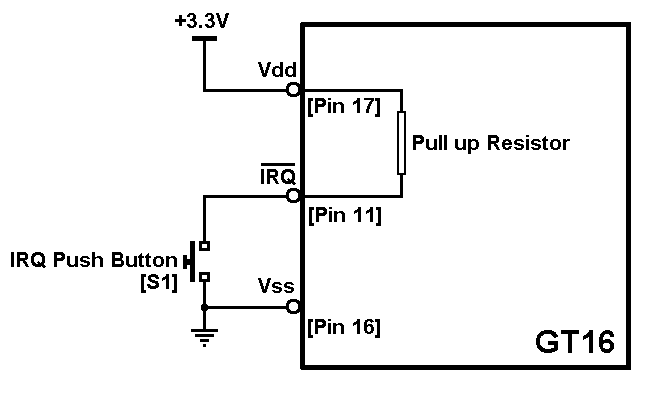
\includegraphics[width=0.7\textwidth]{model.png}
\caption{A block diagram illustrating the connections to the IRQ pin on the MCS08GT16A microcontroller (Please
note that your headings should be short descriptions of what is in the diagram not simply the figure title)}
\label{fig:model}
\end{figure}



\section{Post-development Verification of Specifications}
  Having performed the aforementioned tests on the rover model and the complete software system, a full post-development verification was performed in which each of the requirements as outlined in Section~\ref{subsec:probDef-vehicleSpecifications} were analysed against the final product. The analysis aimed to determine if each requirement was satisfied and this was used as a platform for discussion on the entire design, development and the project in general (thus justifying the lack of a ``Discussions'' section in this report).
  
  \begin{itemize}
    \item \textbf{Mechanical}
    \begin{RM}
      \item General Specifications:
      \begin{RM}
        \item \textbf{Partially Satisfied}\\
        All components of the vehicle were proportional to the 3D reference model \cite{nasa3Dprint} provided by NASA except in the mast and head assembly, whereby the servo and camera dimensions did not allow for smaller components, and in the beams of the suspension system.
        
        \textbf{Proposed improvements:}
        \begin{itemize}
          \item Sourcing of a smaller camera module would allow for a smaller camera head assembly together with better planning of the mounting of the camera inside of the head cavity.
          \item A smaller ultrasonic proximity sensor would alleviate the requirement for the extension of the head canopy for mounting purposes.
        \end{itemize}
      \end{RM}
      \item Body:
      \begin{RM}
        \item \textbf{Fully Satisfied}
        \item \textbf{Fully Satisfied}
        \item \textbf{Fully Satisfied}
        \item \textbf{Fully Satisfied}
        \item \textbf{Fully Satisfied}
        \item \textbf{Fully Satisfied}\\
        Mounting of the DC to DC Converter module and the pulse to analog converters was moved from the body to an additional acrylic piece fastened to the PWM extension module.
        \item \textbf{Fully Satisfied}
      \end{RM}
      \item Mast:
      \begin{RM}
        \item \textbf{Fully Satisfied}
        \item \textbf{Partially Satisfied}\\
        The range of actuation in the servo components chosen for the panning axis rotation of the head was limited to $180^\circ$.
        
        \textbf{Proposed Improvements:}
        \begin{itemize}
          \item Make use of a servo component capable of offering full rotation. This type of servo was not available at the time of design and development of the project.
        \end{itemize}
        \item \textbf{Fully Satisfied}
        \item \textbf{Partially Satisfied}\\
        Using the servo shaft for mounting reduced the structural stability of the assembly due to play in the plastic gears of the component. While the rigidity of the mast and head assembly was well within that which was required for operation, improved rigidity would have been possible with an alternative mounting configuration and/or use of metal gear servos. This is discussed further in Section~\ref{subsec:rec-servoSuitability}.
      \end{RM}
      \item Head:
      \begin{RM}
        \item \textbf{Fully Satisfied}
        \item \textbf{Fully Satisfied}
        \item \textbf{Fully Satisfied}
      \end{RM}
      \item Suspension:
      \begin{RM}
        \item \textbf{Fully Satisfied} as tested in \ref{test:obstacleTest}.
        \item \textbf{Fully Satisfied} as tested in \ref{test:obstacleTest}.
      \end{RM}
      \item Wheels and Hubs/Pivots:
      \begin{RM}
        \item \textbf{Fully Satisfied}
        \item \textbf{Fully Satisfied}
        While the traction capability of the designed wheels was not tested due to lack of a terrain, the wheels replicated the traction pattern on the tires of \textit{Curiosity}.
        \item \textbf{Fully Satisfied} as tested in \ref{test:collisionTest}.
      \end{RM}
    \end{RM}
    
    \item \textbf{Electrical}
    \begin{RE}
      \item Actuation:
      \begin{RE}
        \item \textbf{Fully Satisfied} as tested in \ref{test:stationaryTest} and \ref{test:obstacleTest}.
        \item \textbf{Fully Satisfied} as tested in \ref{test:obstacleTest}.
        \item \textbf{Fully Satisfied}
      \end{RE}
      \item Central Control:
      \begin{RE}
        \item \textbf{Fully Satisfied}
        \item \textbf{Fully Satisfied}
        \item \textbf{Fully Satisfied} as partially tested in \ref{test:collisionTest}.
        \item \textbf{Fully Satisfied}
      \end{RE}
      
      Note that the choice of the Intel Edison was suitable for the designed rover, however, the severely limited control of the GPIO pins and other peripherals such as PWM could have been avoided if another device was chosen. This is further discussed in Section~\ref{subsec:rec-choiceOfRCEBoard}.
      
      \item Power:
      \begin{RE}
        \item \textbf{Fully Satisfied}
        \item \textbf{Fully Satisfied}
        \item \textbf{Fully Satisfied}
        \item \textbf{Fully Satisfied}
        \item \textbf{Fully Satisfied}
        \item \textbf{Fully Satisfied}
      \end{RE}
      \item Sensors:
      \begin{RE}
        \item \textbf{Partially Satisfied}\\
        Due to the limitations in the Intel Edison's ability to measure input electrical pulses, the pulse to analog conversion solution introduced a significant increase in the response time of the distance measurements. This meant that while satisfactory data was acquired, it was not immediate and thus affected the speed of obstacle detection.
        
        \textbf{Proposed Improvements:}
        \begin{itemize}
          \item Source the I$^2$C backpack designed to allow the Intel Edison to correctly interface with the HC-SR04 Sensors.
          \item Source digital proximity sensors or range-finders.
        \end{itemize} 
        \item \textbf{Fully Satisfied}
        \item \textbf{Not Satisfied} as discussed in the analysis of \ref{li:probDef-spec-sensors-immediateObstacleData}.
      \end{RE}
      \item Camera:
      \begin{RE}
        \item \textbf{Fully Satisfied}
        \item \textbf{Partially Satisfied}\\
        Post-manufacture modifications to the head canopy printed part had to be made to allow mounting of the camera. Due to the time-scale of the project, ordering of components and design of the components within the mechanical system had to occur simultaneously. The dimensions of the web camera module were unknown during the design of the mast assembly.
        \item \textbf{Fully Satisfied}
      \end{RE}
  \end{RE}
\end{itemize}
  
\subsubsection{Software System Specifications}
  \begin{itemize}
    \item \textbf{Rover Embedded Software}
    \begin{RS}
      \item General Specifications:
      \begin{RS}
        \item \textbf{Fully Satisfied}
        \item \textbf{Fully Satisfied}
      \end{RS}
      \item Control:
      \begin{RS}
        \item \textbf{Fully Satisfied}
        \item \textbf{Fully Satisfied}
        \item \textbf{Fully Satisfied}
      \end{RS}
      \item Telemetry:
      \begin{RS}
        \item \textbf{Fully Satisfied}
      \end{RS}
      \item Video Stream:
      \begin{RS}
        \item \textbf{Fully Satisfied}
        \item \textbf{Fully Satisfied}
      \end{RS}
    \end{RS}
    
    \item \textbf{Server}
    \begin{RS}[resume]
      \item General Requirements:
      \begin{RS}
        \item \textbf{Fully Satisfied}
        \item \textbf{Fully Satisfied}
        \item \textbf{Fully Satisfied}
        \item \textbf{Fully Satisfied}
      \end{RS}
      \item Video Broadcast:
      \begin{RS}
        \item \textbf{Fully Satisfied}
        \item \textbf{Fully Satisfied} as tested in \ref{test:serverLoadTest}.
        \item \textbf{Fully Satisfied}
      \end{RS}
      \item Data Relay:
      \begin{RS}
        \item \textbf{Fully Satisfied}
        \item \textbf{Partially Satisfied}
        The means by which long distance communication was simulated was rudimentary in that it consisted only of a time delay below 60 seconds. This was not an accurate depiction of the communication dynamic between Earth and \textit{Curiosity}, however, such a simulation would have taken away from the experience of the user.
        \item \textbf{Fully Satisfied}
        \item \textbf{Fully Satisfied}
      \end{RS}
    \end{RS}
      
    \item \textbf{Client}
    \begin{RS}[resume]
      \item General Requirements:
      \begin{RS}
        \item ![Fill out]
      \end{RS}
      \item Control:
      \begin{RS}
        \item \textbf{Fully Satisfied}
      \end{RS}
      \item Telemetry:
      \begin{RS}
        \item \textbf{Fully Satisfied}
      \end{RS}
      \item Video Feed:
      \begin{RS}
        \item \textbf{Fully Satisfied}
      \end{RS}
    \end{RS}
  \end{itemize}

\chapter{Conclusions}
\label{chap:conclusions}
  In recognition of the potential of today's technology, specifically that of interconnectivity of devices and access of resources and services by many more than before, the project aimed to leverage advancements in prototyping, modern manufacture and the web in the design and development of a scaled down, working model of JPL's Mars Curiosity Rover, a major component of the Mars Science Laboratory Mission. The design setting was one whereby the model would be used for education in a modern-style, a highly interactive and accessibly means to allowing users to experience the nature of control of interplanetary rovers and insight into exploration of another planet.
  
  The design initiated with a review of \textit{Curiosity}, its mechanical design and instrumentation as well as supporting fields of engineering and other literature. A comprehensive review of the client requirements was performed to result in a list of technical specification upon which the rest of the design process was based. The project was, at this point, broken into multiple components which followed the design process in parallel. A conceptual design and development procedure was performed within each of the design components and this resulted in the choice of the all technologies and principles for each aspect of each component. The model was then designed in full detail which included a complete and dynamic 3D CAD model of the rover, electrical schematics and a plan of the software architecture. With the design completed, a BOM was drawn up and all components and manufacturing services sourced. The mechanical and electrical systems of the rover were assembled upon receipt of components and the 3D components that were outsourced. Simultaneously, the three software components (RCE, RSVP Server and RSVP Client) were developed and testing of these components was performed throughout the development phase.
  
  After a phase of integration of the developed software components and mechanical and electrical systems, which required multiple iterative developments to be made to all of the systems, the completed model was put through a series of tests which were in accordance with the technical specifications drawn up at the beginning of the project, of which the tests indicated the success of the design in these areas. The model and software system were then analysed against the list of specification which were individually verified. Discussion around specifications that were not fully satisfied led to candidate solutions and suggestions for rectification of any shortfall in the design.
  
  The project concluded with the successful design and development of the model of \textit{Curiosity} which was well suited to an educational environment and exhibited the effectiveness and benefits of modern design, electronics and web technologies in the context of education and outreach. Further developments were made that allowed the project to be open-sourced, making possible the replication of the project and providing insights into methodologies of the design of hardware and software for this type of project.
\chapter{Recommendations and Future Work}
\label{chap:recommendationsAndFutureWork}
  \section{Recommendations}
    \subsection{RCE Hardware Platform}
      As discussed in Section~\ref{subsec:rec-choiceOfRCEBoard}, the Intel Edison exhibited hardware-software limitations which negatively impacted the performance of some of the peripherals. A candidate solution would be to split the responsibility of the RCE between two devices. The Intel Edison performed well for scheduling, communication and video streaming and thus remains a suitable device for those responsibilities. A separate micro-controller module could be designed to accompany the Intel Edison, and would handle control of hardware and acquisition of data from hardware with the required performance and accuracy. The accompanying module could communicate with the Intel Edison via a serial interface such as I$^2$C and potentially alleviate the requirement for the Arduino extension module thus reducing the RCE boards spatial footprint.
      
    \subsection{Web Camera}
      The web camera chosen included many unnecessary features which were not required by the design. It is recommended that a smaller web camera module be used to decrease the required size of the head component and thus bring the camera and head sensor assembly to within proportions.
      
    \subsection{Proximity Sensors}
      The HC-SR04 ultrasonic sensors provided accurate proximity measurements, but were large in comparison to the majority of the body components. A smaller proximity sensor device would dominate less the overall aesthetic of the rover. If the Intel Edison is to be used for data acquisition, a proximity sensor with a digital interface would benefit the design.
      
    \subsection{Drive Servos}
      It is recommended to use servos designed for continuous rotation to ensure stability of the mounting of wheels. Servos with metal gears would also bring torque and robustness benefits to the driving of the wheels and the rover's traversal capabilities in general.
      
  \section{Future Work}
    \subsection{Rover Model as Mission and Operations Test Bed}
      During the development of the rover model, it became apparent that the model could be used in a more scientific manner. The rover could be used as a test bed for many of the systems and software algorithms for all aspects of the operation of this type of exploratory vehicle. This might include the testing of path planning algorithms or perhaps newly developed optical obstacle detection and avoidance systems with supporting automation.
      
    \subsection{Martian Environment Simulation}
    \label{subsec:fut-martianEnvironmentSimulation}
      As an extension to the project, research on methods of developing small scale and low-cost but accurate Martian environments could be done to support test-bed-like applications of such a rover model as well as improve the educational value and user engagement when operating the rover.
    
    \subsection{Steroscopic Video Feed}
      While the rover model in this project only required a monoscopic video stream, some of the cameras on \textit{Curiosity} are placed in pairs to provide stereoscopic imagery of the subject. This was designed for extraction of depth data as well as for operator immersion. A second camera could be added to the rover model in this project, along with modifications to the RCE board to allow for a second camera input, to provide a similar experience to the visualisation component of the RSVP used at JPL. 
    
    \subsection{Direct Control Capabilities}
      While it was deemed acceptable for the system to rely on a central server endpoint for the operation of the rover model in this project, improvements to the accessibility of operation could be achieved by designing a second mode of operation in which the server component of the software system is removed and the RSVP Clients communicate directly with the RCE system. The platform or device hosting the RSVP Client would connect to the RCE Board's wireless access point and the RCE would offer server endpoint functionality and video broadcast. Investigations into the performance limitations as a result would need to be made.
      
    \subsection{Improved RoSE Sequencing Editing}
      The RoSE control interface in this project was greatly simplified due to lack of time. Improvements could be made to the editor component of the RSVP Client UI such as the ability to organise sequences into folders or groups, save sequences or portions thereof for later use and the addition of many other commands for operation of all aspects of the rover.
    
    \subsection{Hardware Feedback Telemetry}
      Currently, the rover model does not have the ability to report the actual hardware states due to lack of sensors and other electronics required to obtain such data. The rover model could be extended to include sensors to provide more accurate state data to the RSVP Client and even to the RCE itself which could be used to improve the control of hardware and implement proper fault detection.

\bibliography{references}
\appendix
\chapter{List of Contributory Open Source Projects}
\label{appendix:openSourceList}

Add any information here that you would like to have in your project but is not necessary in the main
text. Remember to refer to it in the main text. Separate your appendices based on what they are for
example. Equation derivations in Appendix A and code in Appendix B etc.

\chapter{Contents of Submitted DVD}
  A DVD was submitted to accompany this report consisting of supporting material for the project. Below is an outline of the file structure of the disk as well as a description of the material.
  
  \begin{itemize}
    \item \textbf{Folder - \mintinline{js}{cad}:} A complete, packed set of files containing the entire 3D CAD design.
    \item \textbf{Folder - \mintinline{js}{media}:}
      \begin{itemize}
        \item \textbf{Folder - \mintinline{js}{renders}:} 3D renders of the completed rover model rendered in the 3D CAD software used for the project.
        \item \textbf{Folder - \mintinline{js}{images}:} Images of the completed rover model.
        \item \textbf{Folder - \mintinline{js}{screenshots}:} Screenshots of the completed RSVP Client user interface.
      \end{itemize}
    \item \textbf{Git Repository - \mintinline{js}{mars-rover-writeup}:} The \LaTeX~source for this report. Also available online at \url{https://github.com/WoodyWoodsta/mars-rover-rce/tree/thesis}.
    \item \textbf{Folder - \mintinline{js}{software}:} Note that the versions of the software in the repositories listed below are available as a frozen version on the \mintinline{js}{thesis} branch. Continued development of the software is kept on other branches including \mintinline{js}{master}.
      \begin{itemize}
        \item \textbf{Git Repository - \mintinline{js}{mars-rover-rce}:} The software project and source used for the RCE. Also available online at \url{https://github.com/WoodyWoodsta/mars-rover-rce/tree/thesis}.
        \item \textbf{Git Repository - \mintinline{js}{mars-rover-rsvp-server}:} The software project and source used for the RSVP Server. Also available online at \url{https://github.com/WoodyWoodsta/mars-rover-rsvp-server/tree/thesis}.
        \item \textbf{Git Repository - \mintinline{js}{mars-rover-rsvp-client}:} The software project and source used for the RSVP Client. Also available online at \url{https://github.com/WoodyWoodsta/mars-rover-rsvp-client/tree/thesis}.
      \end{itemize}
    \item \textbf{File - \mintinline{js}{mars-rover-writup.pdf}:} This report, in PDF format.
    \item \textbf{File - \mintinline{js}{mars-rover-demonstration.mp4}:} A demonstration video showing some of the tests performed on the final rover model.
  \end{itemize}

\end{document}

%\begin{figure}[ht]
%\centering
%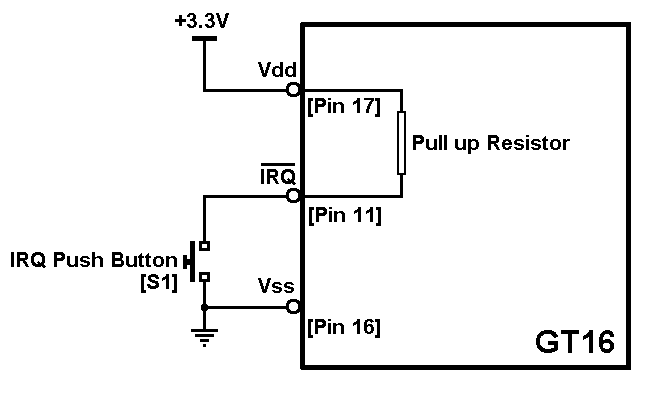
\includegraphics[width=0.7\textwidth]{model.png}
%\label{fig:model}
%\caption{A block diagram illustrating the connections to the IRQ pin on the MCS08GT16A microcontroller (Please
%note that your headings should be short descriptions of what is in the diagram not simply the figure title)}
%\end{figure}

